\chapter{Experimental Setup and Results}

\section{Experimental Setup}
\label{sec:experimentalsetup}

Although the algorithms developed in this thesis are aimed at dynamic
environments, for the sake of completeness they will also be compared in
partially known environments and in totally unknown environments, where some or
all of the obstacles become visible to the planner as the robot approaches each
one of them, simulating a robot with limited sensor range.

\subsection{Dynamic Environment}

The first environment for our experiments consists on two maps with 30~moving
obstacles the same size of the robot, with a random speed between 10\% and 55\%
the speed of the robot. Good performance in this environment is the main focus
of this thesis. This \emph{dynamic environments} are illustrated in figures~%
\ref{fig:office-dynamic} and~\ref{fig:800-dynamic}.

\begin{figure}[h!]
\begin{center}
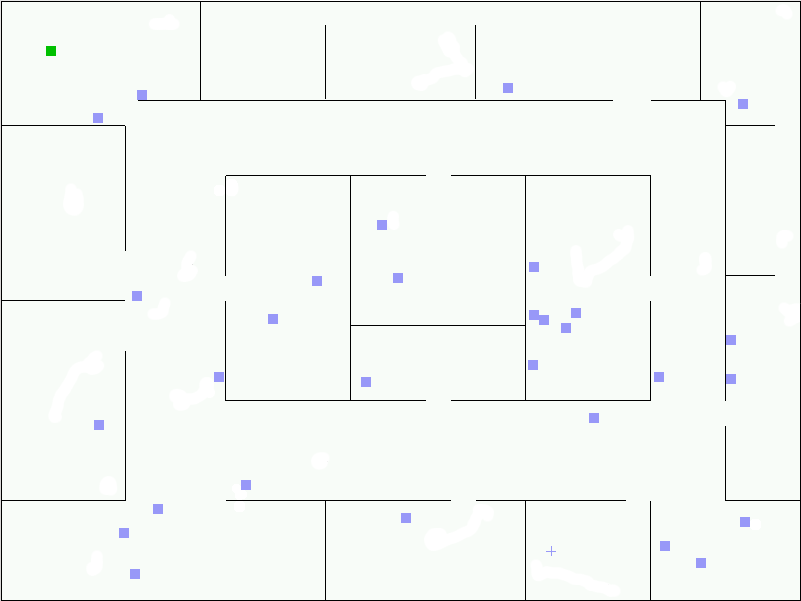
\includegraphics[width=0.7\textwidth]{images/office-dynamic}
\caption[The dynamic environment, map 1]{The dynamic environment, map 1. The \emph{green} square is our robot,
currently at the start position. The
\emph{blue} squares are the moving obstacles. The \emph{blue} cross is the goal.}
\label{fig:office-dynamic}
\end{center}
\end{figure}

\begin{figure}[h!]
\begin{center}
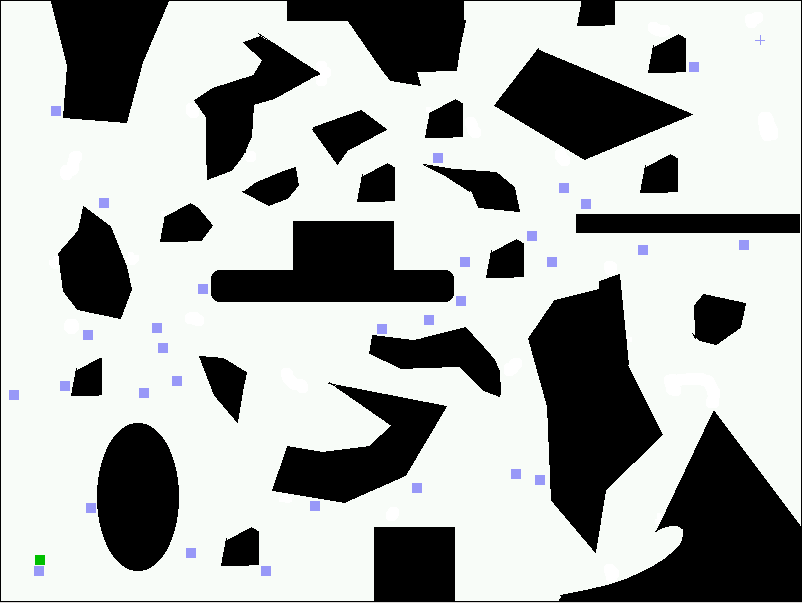
\includegraphics[width=0.7\textwidth]{images/800-dynamic}
\caption[The dynamic environment, map 2]{The dynamic environment, map 2. The \emph{green} square is our robot,
currently at the start position. The
\emph{blue} squares are the moving obstacles. The \emph{blue} cross is the goal.}
\label{fig:800-dynamic}
\end{center}
\end{figure}

\subsection{Partially Known Environment}

The second environment uses the same maps, but with a few  obstacles, three to four
times the size of the robot, that become visible when the robot approaches each
one of them. This is the kind of environment that most dynamic RRT variants were designed
for. The
\emph{partially known environments} are illustrated in figure~\ref{fig:office-partial}
and~\ref{fig:800-partial}.

\begin{figure}[h!]
\begin{center}
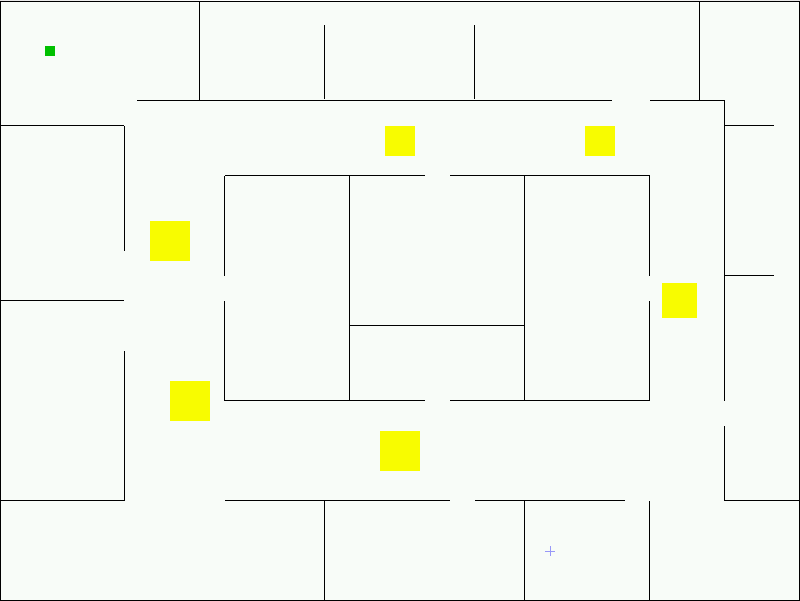
\includegraphics[width=0.7\textwidth]{images/office-partial}
\caption[The partially known environment, map 1]{The partially known environment, map 1. The \emph{green} square is our robot,
currently at the start position. The \emph{yellow} squares are the suddenly
appearing obstacles. The \emph{blue} cross is the goal.}
\label{fig:office-partial}
\end{center}
\end{figure}

\begin{figure}[h!]
\begin{center}
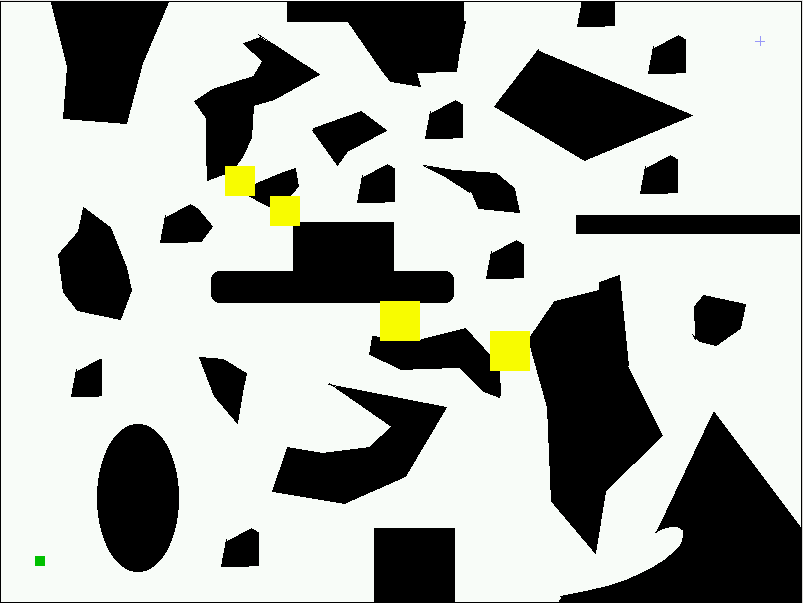
\includegraphics[width=0.7\textwidth]{images/800-partial}
\caption[The partially known environment, map 2]{The partially known environment, map 2. The \emph{green} square is our robot,
currently at the start position. The \emph{yellow} squares are the suddenly
appearing obstacles. The \emph{blue} cross is the goal.}
\label{fig:800-partial}
\end{center}
\end{figure}

\subsection{Unknown Environment}

For completeness sake, we will compare the different technique in a third
environment, were we use one of  the maps presented before, but
all the obstacles will initially be unknown to the 
planners, and will become visible as the robot approaches them, forcing several
re-plans. This \emph{unknown environment} is illustrated in figure~%
\ref{fig:office-unknown}.


\begin{figure}[h!]
\begin{center}
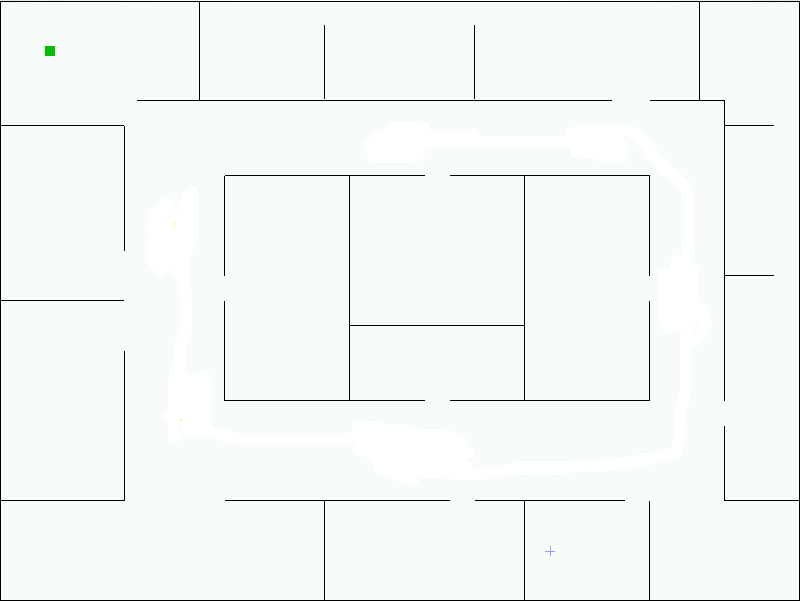
\includegraphics[width=0.7\textwidth]{images/office-unknown}
\caption[The unknown environment]{The unknown environment. The \emph{green} square is our robot,
currently at the start position. The \emph{blue} cross is the goal. None of the
obstacles is visible initially to the planners}
\label{fig:office-unknown}
\end{center}
\end{figure}

\section{Implementation Details}

The algorithms where implemented in C++ using the MoPa framework%
\footnote{MoPa homepage:
\texttt{https://csrg.inf.utfsm.cl/twiki4/bin/view/CSRG/MoPa}}
 partly developed by the author. This framework features exact collision
 detection, three different map formats (including \texttt{.pbm} images from any
 graphic editor), dynamic, unknown
 and partially known environments and support for easily adding new planners.
 One of the biggest downsides is that it only supports rectangular objects, so
 several objects must be used to represent other geometrical shapes, as in
 figure~\ref{fig:800-partial}, composed of 1588 rectangular objects.

There are several variations that can be found in the literature when
implementing RRT. For all our RRT variants, the following are the details on
where we departed from the basics:
\begin{enumerate}
\item We always use two trees rooted at $q_{init}$ and $q_{goal}$.
\item Our EXTEND function, if the point cannot be added without collisions to a
tree, adds the mid point between the nearest tree node and the nearest collision
point to it.
\item In each iteration, we try to add the new randomly generated point to both
trees, and if successful in both, the trees are merged, as proposed in~%
\cite{Kuffner00}.
\item\label{sec:advance} We believe that there might be significant performance 
differences between allowing or not allowing the robot to
advance towards the node nearest to the goal when the trees are disconnected, as
proposed in~\cite{Zucker07}. 
\end{enumerate}
In point~\ref{sec:advance} above, the problem is that the robot would become stuck
if it enters a small concave zone of the environment (like a room in a building)
while there are moving obstacles inside that zone, but otherwise it can lead to
better performance. Therefore we present results for both kinds of behavior:
DRRT-adv and MP-RRT-adv move even when the trees are disconnected, while
DRRT-noadv and MP-RRT-noadv only
move when the trees are connected.

In MP-RRT, the forest was handled by simply replacing the oldest tree in it if the
forest had reached the maximum allowed size.

Concerning the parameter selection, the probability for selecting a point in the
vicinity of a point in the waypoint cache in DRRT was set to 0.4 as suggested in~%
\cite{Ferguson06}. The probability for trying to reuse a subtree in
MP-RRT was set to 0.1 as suggested in~\cite{Zucker07}.
Also, the forest size was set to 25 and the minimum size of a
tree to be saved in the forest was set to 5 nodes.

For the combined RRT-EP/N, it was considered the planner was stuck after two
seconds without a feasible solution in the population, at which point a
new solution from a RRT variant is inserted into the population. For the simple
multi-stage probabilistic algorithm, the restart is made after one second of
encountering the same obstacle along the planned path. This second approach,
which seems better, cannot be applied to the RRT-EP/N, because there is no
single path to check for collisions, but instead a population of paths. The
restart times where manually tuned.

\section{Results}
\label{sec:results}
The three algorithms were run a hundred times in each
environment and map combination.
The cutoff time was five minutes for all tests, after which the robot was
considered not to have reached the goal. Results are presented concerning:
\begin{itemize}
\item {\it Success rate (S.R.):} The percentage of times the robot arrived at the goal,
before reaching the five minutes cutoff time. This does not account for
collisions or time the robot was stopped waiting for a plan.
\item {\it Number of nearest neighbor lookups performed by each algorithm (N.N.):} One of the
possible bottlenecks for tree-based algorithms
\item {\it Number of collision checks performed (C.C.),} which in our specific
implementation takes a significant percentage of
the running time
\item {\it Time} it took the robot to reach the goal, $\pm$ the standard
deviation.
\end{itemize}

\subsection{Dynamic Environment Results}
The results in tables~\ref{table:dynamic1} and~\ref{table:dynamic2} show that
the multi-stage algorithm takes considerably less time than the DRRT 
and MP-RRT to reach
the goal, with far less collision checks. The combined RRT-EP/N is a close
second. It was expected that nearest neighbor
lookups would be much lower in both combined algorithms than in the RRT variants,
because they are only performed in the initial phase and restarts, 
not during navigation.
The combined algorithms produce more consistent results
within a map,
as shown by their smaller standard deviations, but also across different
maps. An interesting fact is that in map~1 DRRT is slightly faster than MP-RRT, and
in map~2 MP-RRT is faster than DRRT. However the differences are too small to
draw any conclusions.
Figures~\ref{fig:times} and~\ref{fig:success-rate} show the times and
success rates of the different algorithms, when changing the number of dynamic
obstacles in map~1. The simple multi-stage algorithm and the mixed RRT-EP/N
clearly show the best performance, while the DRRT-adv and MP-RRT-adv
significantly reduce their success rate when confronted to more than 30~moving
obstacles. 



\begin{table}[h!]
\caption{Dynamic Environment Results, map 1.}
\label{table:dynamic1}
\centering
\begin{tabular}{|l||r|r|r|r@{$\ \pm\ $}l|}
\hline
\textbf{Algorithm} & \textbf{S.R.[\%]} & \textbf{C.C.} & \textbf{N.N.} &
\multicolumn{2}{c|}{\textbf{Time[s]}}\\
\hline
Multi-stage & 99 & 23502 & 1122 & 6.62 & 0.7\\
\hline
RRT-EP/N & 100 & 58870 & 1971 & 10.34 & 14.15 \\
\hline
DRRT-noadv & 100 & 91644 & 4609 & 20.57 & 20.91\\
\hline
DRRT-adv & 98 & 107225 & 5961 & 23.72 & 34.33\\
\hline
MP-RRT-noadv & 100 & 97228 & 4563 & 22.18 & 14.71\\
\hline
MP-RRT-adv & 94 & 118799 & 6223 & 26.86 & 41.78\\
\hline
\end{tabular}
\end{table}

\begin{table}[h!]
\caption{Dynamic Environment Results, map 2.}
\label{table:dynamic2}
\centering
\begin{tabular}{|l||r|r|r|r@{$\ \pm\ $}l|}
\hline
\textbf{Algorithm} & \textbf{S.R.[\%]} & \textbf{C.C.} & \textbf{N.N.} &
\multicolumn{2}{c|}{\textbf{Time[s]}}\\
\hline
Multi-stage & 100 & 10318 & 563 & 8.05 & 1.47\\
\hline
RRT-EP/N & 100 & 21785 & 1849 & 12.69 & 5.75 \\
\hline
DRRT-noadv & 99 & 134091 & 4134 & 69.32 & 49.47\\
\hline
DRRT-adv & 100 & 34051 & 2090 & 18.94 & 17.64\\
\hline
MP-RRT-noadv & 100 & 122964 & 4811 & 67.26 & 42.45\\
\hline
MP-RRT-adv & 100 & 25837 & 2138 & 16.34 & 13.92\\
\hline
\end{tabular}
\end{table}


\begin{figure}[h!]
\begin{center}
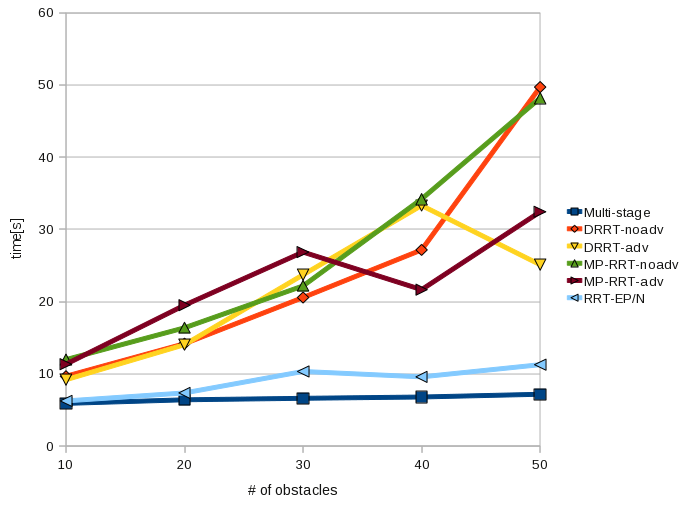
\includegraphics[width=0.9\textwidth]{images/times}
\caption[Dynamic environment time]{Times for different number of moving obstacles in map 1.}
\label{fig:times}
\end{center}
\end{figure}

\begin{figure}[h!]
\begin{center}
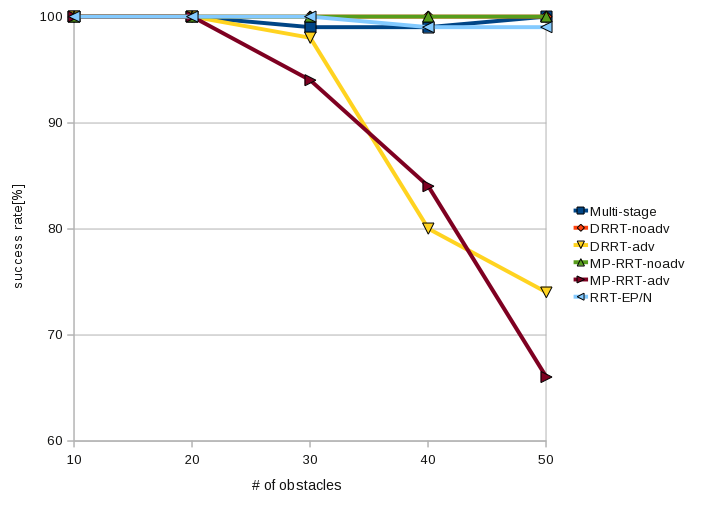
\includegraphics[width=0.9\textwidth]{images/success-rate}
\caption[Dynamic environment success rate]{Success rate for different number of moving obstacles in
map 1.}
\label{fig:success-rate}
\end{center}
\end{figure}

\subsection{Partially Known Environment Results}
Taking both maps into consideration, the results in tables~\ref{table:partial1}
and~\ref{table:partial2} 
show that both combined algorithms are faster and more consistent than the RRT
variants, with the simple multi-stage algorithm being faster in both. 
These results were unexpected, as the combined algorithms were designed
for dynamic environments.
It is
worth to notice though, that
in map~1 DRRT-adv is a close second, but in map~2 it is a close last, so its
lack of reliability does not make it a good choice in this scenario. In this
environment, as in the dynamic environment, in map~1 DRRT is faster than MP-RRT,
while the opposite happens in map~2.

\begin{table}[h!]
\caption{Partially Known Environment Results, map 1.}
\label{table:partial1}
\centering
\begin{tabular}{|l||r|r|r|r@{$\ \pm\ $}l|}
\hline
\textbf{Algorithm} & \textbf{S.R.[\%]} & \textbf{C.C.} & \textbf{N.N.} &
\multicolumn{2}{c|}{\textbf{Time[s]}}\\
\hline
Multi-stage & 100 & 12204 & 1225 & 7.96 & 2.93\\
\hline
RRT-EP/N & 99 & 99076 & 1425 & 9.95 & 2.03 \\
\hline
DRRT-noadv & 100 & 37618 & 1212 & 11.66 & 15.39\\
\hline
DRRT-adv & 99 & 12131 & 967 & 8.26 & 2.5\\
\hline
MP-RRT-noadv & 99 & 49156 & 1336 & 13.82 & 17.96\\
\hline
MP-RRT-adv & 97 & 26565 & 1117 & 11.12 & 14.55\\
\hline
\end{tabular}
\end{table}

\begin{table}[h!]
\caption{Partially Known Environment Results, map 2.}
\label{table:partial2}
\centering
\begin{tabular}{|l||r|r|r|r@{$\ \pm\ $}l|}
\hline
\textbf{Algorithm} & \textbf{S.R.[\%]} & \textbf{C.C.} & \textbf{N.N.} &
\multicolumn{2}{c|}{\textbf{Time[s]}}\\
\hline
Multi-stage & 100 & 12388 & 1613 & 17.66 & 4.91\\
\hline
RRT-EP/N & 100 & 42845 & 1632 & 22.01 & 6.65 \\
\hline
DRRT-noadv & 99 & 54159 & 1281 & 32.67 & 15.25\\
\hline
DRRT-adv & 100 & 53180 & 1612 & 32.54 & 19.81\\
\hline
MP-RRT-noadv & 100 & 48289 & 1607 & 30.64 & 13.97\\
\hline
MP-RRT-adv & 100 & 38901 & 1704 & 25.71 & 12.56\\
\hline
\end{tabular}
\end{table}

\subsection{Unknown Environment Results}

Results in table~\ref{table:unknown} present the combined RRT-EP/N clearly as
the faster algorithm in unknown environments, with the multi-stage algorithm in
second place. In contrast to dynamic and partially known environments in this
same map, MP-RRT is faster than DRRT.

\begin{table}[h!]
\caption{Unknown Environment Results}
\label{table:unknown}
\centering
\begin{tabular}{|l||r|r|r|r@{$\ \pm\ $}l|}
\hline
\textbf{Algorithm} & \textbf{S.R.[\%]} & \textbf{C.C.} & \textbf{N.N.} &
\multicolumn{2}{c|}{\textbf{Time[s]}}\\
\hline
Multi-stage & 100 & 114987 & 2960 & 13.97 & 3.94\\
\hline
RRT-EP/N & 100 & 260688 & 2213 & 10.69 & 2.08 \\
\hline
DRRT-noadv & 98 & 89743 & 1943 & 18.38 & 22.01\\
\hline
DRRT-adv & 100 & 104601 & 2161 & 19.64 & 34.87\\
\hline
MP-RRT-noadv & 99 & 129785 & 1906 & 21.82 & 27.23\\
\hline
MP-RRT-adv & 100 & 52426 & 1760 & 16.05 & 10.87\\
\hline
\end{tabular}
\end{table}
